%!TEX root = ../Main.tex

\chapter{Genetic map of \textit{Yr15} with RNA-Seq}
\chaptermark{Genetic map of \textit{Yr15}}
\label{yr15}
%This section describes in detail than the paper of \citet{Ramirez-Gonzalez-2014}
 
%Breeding importance of \textit{Yr15} and original source (an introgression of \textit{T. diccocoides}). 
Wheat breeding programs aim to improve the wheat lines available for production.
One way to facilitate the selection of elite lines is to find molecular markers that can facilitate the selection of seeds without having to wait until the phenotype is observed.   
Bulk Segregant Analysis (BSA) consists on pooling the DNA of individuals with contrasting phenotypes \citep{Michelmore1991} on a segregating population. 
The bulks show as heterozygous except for the region that is linked to the trait of interest. 
This approach can be used to identify SNPs using High Throughput Sequencing, such as: exome capture \citep{Hodges2007}, RNA-Seq \citep{Pickrell2010}, whole genome resquencing \citep{Schneeberger2009}, among others. 

One of the traits desired in an elite line is the resistance to pathogens, such as \textit{Puccinia striiformis} f. sp.  \textit{tritici}, the fungi responsible of yellow rust.
A source of resistance genes is are introgressions from other species, suchas \textit{Triticum diccocides}. 
In the University of Sydney a collection of Near Isogenic Lines (NILs) with introgressions to several Yellow Rust resistance genes on a susceptible background were developed \citep{Wellings1998}. 
On this chapter the NIL for the \textit{Yr15} locus is used to produce a mapping population to improve diagnostic markers. 
The population was sequenced using RNA-Seq and a bioinformatic pipeline was developed to score Single Nucleotide Polymorphisms (SNPs) linked to the \textit{Yr15} locus.  
Finally, the best candidate SNPs where selected to produce a genetic map which lead to a triplet of markers diagnostic to the target locus. The steps described in this chapter were first published in \citet{Ramirez-Gonzalez2015c} and the results of this chapter are published in \citet{Ramirez-Gonzalez2015b}.

\section{Mapping population}


\begin{figure}
%\begin{wrapfigure}[17]{R!}{7cm}
    \centering
     
     \begin{subfigure}[b]{0.4\textwidth}
        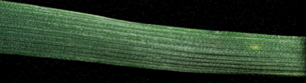
\includegraphics[width=1\textwidth]{Yr15/Figures/population/Yr15Photo.png}
        \caption{}
        \label{fig:yr15.yr15Photo}
    \end{subfigure}
    ~
    \begin{subfigure}[b]{0.4\textwidth}
        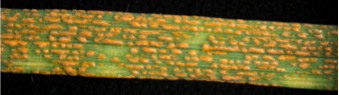
\includegraphics[width=1\textwidth]{Yr15/Figures/population/AVSPhoto.png}
        \caption{}
        \label{fig:yr15:avsPhoto}
    \end{subfigure}

     \begin{subfigure}[b]{0.8\textwidth}
        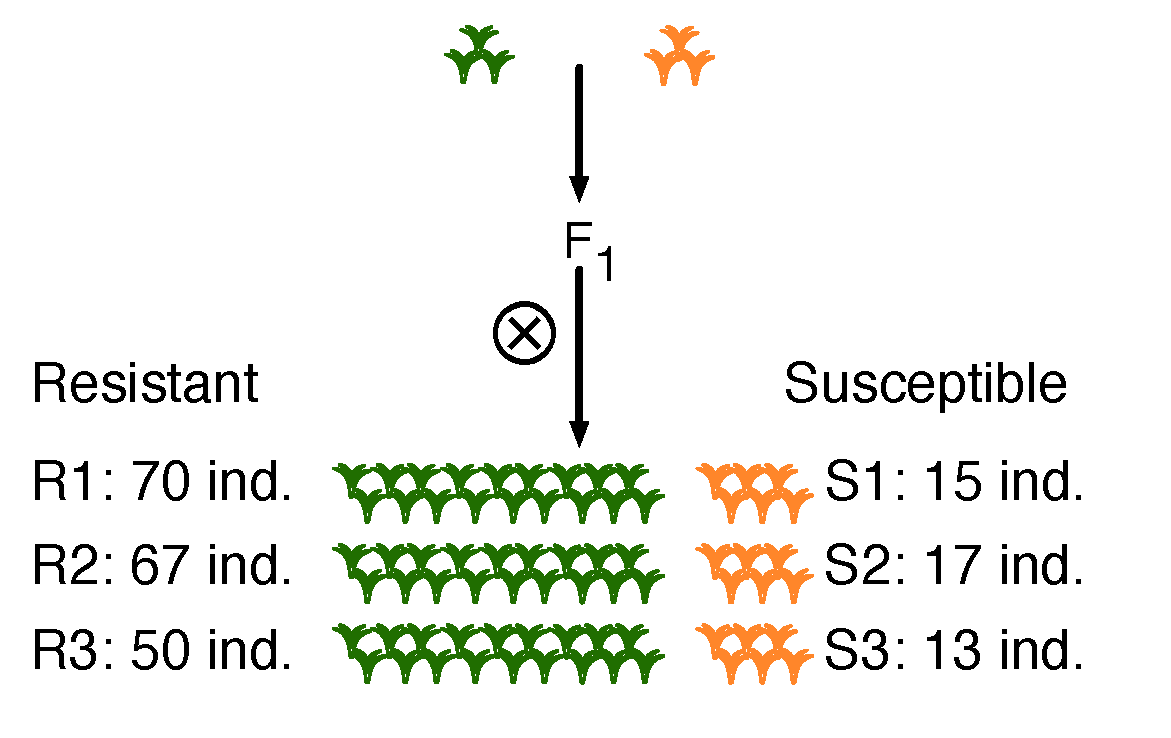
\includegraphics[width=1\textwidth]{Yr15/Figures/population/F2Population.pdf} 
    \caption{ }
    \label{fig:yr15:f2}
	\end{subfigure}

    \caption{Response of (\subref{fig:yr15.yr15Photo}) Avocet + \textit{Yr15} and (\subref{fig:yr15:avsPhoto}) Avocet when inoculated with \textit{Puccinia striiformis} f. sp.  \textit{tritici} at the three leaf stage. (\subref{fig:yr15:f2}) The phenotype of the $F_{2}$ population was used to produce 6 bulks, 3 resistant and 2 susceptible. The RNA was pooled in bulks accordingly. }

%\end{wrapfigure}
\end{figure}

The population was developed by crossing the resistant line `Avocet + \textit{Yr15}` (\textit{Yr15}) \citep{Wellings1998}, Figure \ref{fig:yr15.yr15Photo}, to the susceptible line Avocet (AVS), Figure \ref{fig:yr15:avsPhoto}. 
$F_{2}$ seeds from tree independent $F_{1}$ plants where sown and tissue was collected, before the fungal inoculation to avoid the effect of the response on the gene expression.  
The plants were challenged at the three leaf stage as it is know that \textit{Yr15} confers resistance in seedlings \citep{Gerechter-Amitai1989}.
The expected segregation on an $F_{2}$ population is 3:1 (resistant:susceptible), since \textit{Yr15} is a dominant gene.
From the 232 plants in the $F_{2}$ population that germinated, 187 were resistant and 45 were susceptible, which deviates slightly from the expected ratio ($\chi^{2}=0.049$).
Segregation distortion has been shown for the same \textit{Yr15} donnor \citep{Randhawa2009}, however the decresed number of succeptible plants can be explained by escapes in the virulence essays (i.e. plants scored as resistant without the \textit{Yr15} locus).   For this study we extracted DNA from individual plants in the $F_{2}$ population and we bulked RNA on 6 different bulks: 3 resistant and, 3 succeptible, Figure \ref{fig:yr15:f2}. 

\section{Sequencing and mapping} 

RNA-Seq and the decision to call SNPs on gene models rather than the whole reference.  Details of the mapping against the Wheat UniGenes \cite{PontiusJUWagnerL2002} and the UCW. \cite{Krasileva2013} gene models.  

\section{SNP Calling}. 
\verb|Ruby| implementation of the methodology described by \citet{Trick2012}. 

\section{Bulk Frequency Ratios} 
Results of the simple SNP calls from the progenitors and how the score of the Bulk Frequency Ratios(BFR) improve the location of the SNPs. 

\section{\textit{In silico} mapping}
Mapping of the gene models to the IWGSC CSS \cite{Mayer2014} reference and the location of the SNPs using the genetic map from \citet{Wang2014}.

\section{Assay selection}. 
The selection criteria to decide which SNPs where selected to produce the genetic map: BFR$>$6, in the short arm of chromosome group 1 and from the \textit{Yr15} progenitor.

\section{Genetic map} 
\label{yr15:geneticMap}
The three versions of the genetic map: With a subset of the F\textsubscript{2} population

\section{Assembly of the transcriptome} 
A comparison between thef known unigenes and the transcript from the progenitors. Since \textit{Yr15} comes from an introgression with \textit{T. diccocoides}, some novel transcripts can be extracted. Analysis of the gels from Mitaly? 

\section{Conclusions} 
Remarks on how this techinque can be used to do fine-mapping and that if I were to start the project now I would  use exome capture or Ren-Seq. 